\documentclass{article}

% ICML 2025 style
\usepackage{icml2025}

% Additional packages
\usepackage{booktabs}
\usepackage{graphicx}
\usepackage{amsmath}
\usepackage{amssymb}
\usepackage{url}
\usepackage{hyperref}
\usepackage{microtype}

% If your build uses biblatex, comment out icml2025 bib style below
% and use \addbibresource{references.bib} + \printbibliography

\icmltitlerunning{When Does a Benchmark Saturate?}

\begin{document}

\twocolumn[
\icmltitle{When Does a Benchmark Saturate? Detecting Regime Shifts in ML Leaderboard Performance Variance}

\begin{icmlauthorlist}
\icmlauthor{Anonymous}{anon}
\end{icmlauthorlist}

\icmlaffiliation{anon}{Anonymous Institution}

\icmlcorrespondingauthor{Anonymous}{anonymous@review.com}

\icmlkeywords{benchmark saturation, change-point detection, PELT, Papers With Code, leaderboard analysis}

\vskip 0.3in
]

\printAffiliationsAndNotice{\icmlEqualContribution}

\begin{abstract}
ML benchmarks lose their ability to discriminate between methods once the community has converged on high-performing approaches --- yet decisions about when to retire them remain informal and subjective. We show that benchmark saturation is not a gradual decline but a discrete structural break: among 115 Papers With Code benchmarks, PELT change-point detection on OLS-detrended residual coefficient of variation identifies a statistically significant regime shift at $\text{paper\_count}^* \approx 39$ (permutation $p=0.035$, piecewise $F$-test $p=0.0021$). Before this threshold, performance variance is nearly $4\times$ higher than the global baseline; after it, variance collapses by 80\% --- consistent with Goodhart saturation dynamics, where community convergence on dominant approaches compresses the score distribution toward a ceiling. Three independently designed experiments corroborate this two-regime structure (pre-regime $F$ $p=0.0009$, post-regime Brown-Forsythe $p=0.0099$). Our results provide the first data-driven, paper-count-based structural break threshold for PwC benchmarks, offering a lightweight, reproducible tool that any leaderboard curator can run on existing data to flag mature benchmarks for retirement review.
\end{abstract}


\section{Introduction}

Among 115 Papers With Code benchmarks, a benchmark's competitive landscape undergoes a discrete phase transition --- not a gradual fade --- at approximately 39 competing papers. Before this threshold, performance scores vary nearly $4\times$ more than the global baseline as the community searches for winning approaches. After it, variance collapses by 80\%. This structural break, detectable in two minutes of computation, offers a principled, quantitative answer to a question the ML evaluation community has long debated informally: when should we retire a benchmark?

The need for benchmark retirement criteria is not merely academic. When a benchmark saturates --- when top models differ by fractions of a percent --- it can no longer rank research contributions meaningfully. Continuing to optimize such benchmarks exemplifies Goodhart's Law at scale: once a measure becomes a target, it ceases to be a good measure~\cite{Goodhart1975}. Yet retirement decisions in the ML community remain largely informal, driven by qualitative consensus rather than quantitative evidence~\cite{Bowman2021}.

Prior work has characterized benchmark saturation in aggregate. Liao et al.~\cite{Liao2022} documented near-saturation trends across 3,765 benchmarks using time-based metrics and coefficient of variation (CoV). The $S_{\text{index}}$~\cite{Akhtar2026} provides a composite saturation score for LLM benchmarks. These contributions establish that saturation is a systemic phenomenon --- but they do not answer the retirement question quantitatively: \textit{at what point in a benchmark's publication history does saturation onset occur?}

We address this gap by reframing benchmark saturation as a structural break detection problem. Our key insight is that benchmark performance variance does not decline gradually --- it undergoes a statistically significant regime shift at a detectable paper\_count threshold. Rather than fitting a monotonic trend to CoV-vs-paper\_count data, we apply PELT change-point detection~\cite{Killick2012} to OLS-detrended residual CoV, directly targeting the transition between exploration and saturation regimes. Two independent tests --- a permutation test on breakpoint position ($p=0.035$) and a piecewise $F$-test comparing one-segment vs.\ two-segment linear models ($p=0.0021$) --- both confirm this transition at $\text{paper\_count}^* \approx 39$.

\textbf{Contributions.} Building on this insight, we make three contributions:

\begin{enumerate}
\item \textbf{Empirical (novel threshold).} We report the first detected structural break in PwC benchmark residual CoV at $\text{paper\_count}^* \approx 39$ ($N=115$ benchmarks, Aug 2026 snapshot), providing a quantitative, paper-count-based candidate threshold for benchmark retirement flagging. This threshold is not available in prior work.

\item \textbf{Empirical (two-regime structure).} We characterize the two regimes: a high-variance exploration phase (pre-breakpoint variance $3.81\times$ global baseline, $F$ $p=0.0009$) and a low-variance saturation phase (post-breakpoint variance $0.20\times$ pre-breakpoint, Brown-Forsythe $p=0.0099$). Three independently designed experiments converge on the same two-regime narrative.

\item \textbf{Methodological.} We demonstrate that PELT on OLS-detrended residual CoV is a viable, computationally efficient, and interpretable approach for detecting saturation onset in benchmark leaderboard data. The methodology is dataset-agnostic, fully automated, and reproducible.
\end{enumerate}

We organize the paper as follows. Section~\ref{sec:related} reviews related work. Section~\ref{sec:method} describes our methodology. Section~\ref{sec:setup} presents experimental setup. Section~\ref{sec:results} reports results. Section~\ref{sec:discussion} discusses interpretation and limitations. Section~\ref{sec:conclusion} concludes.


\section{Related Work}
\label{sec:related}

\subsection{Benchmark Saturation Studies}

The saturation of ML benchmarks has attracted growing attention. Bowman and Dahl~\cite{Bowman2021} argue that standard NLU benchmarks have largely saturated and call for principled retirement criteria --- but their analysis is qualitative; they identify the \textit{need} for criteria without providing a quantitative threshold.

Liao et al.~\cite{Liao2022} conduct the largest systematic study of benchmark saturation, analyzing near-saturation trends across 3,765 benchmarks using time-based metrics and CoV. Their analysis confirms saturation is a systemic phenomenon --- but their metric is time-based (years to saturation), not paper\_count-based, and targets aggregate trends rather than discrete structural breaks.

Akhtar et al.~\cite{Akhtar2026} introduce the $S_{\text{index}}$, a composite saturation metric for 60 LLM benchmarks, characterizing saturation as a continuous property. It does not apply change-point detection to PwC-internal CoV-vs-paper\_count data and does not produce a paper\_count threshold. Vasudevan et al.~\cite{Vasudevan2022} analyze ImageNet saturation in depth, documenting that top-1 accuracy above 90\% no longer discriminates between models --- providing independent evidence for the exploration-phase variance of pre-saturation benchmarks. Cao and Zhao~\cite{Cao2025} demonstrate that LLM benchmark scores are increasingly inflated by test-set pretraining, further motivating saturation detection.

\textbf{The gap:} No prior work applies change-point detection to PwC-internal CoV-vs-paper\_count data to produce a discrete, paper-count-based retirement threshold.

\subsection{Change-Point Detection Methods}

PELT (Pruned Exact Linear Time)~\cite{Killick2012} is an exact dynamic programming algorithm for detecting an unknown number of change-points in 1D signals with a penalized cost function. Wang, Lin and Willett~\cite{Wang2019} establish the VPWBS algorithm's $O_p(1/n)$ localization rate for regression change-points, providing theoretical grounding for PELT's performance at small sample sizes (our $N=115$). The \texttt{ruptures} Python library~\cite{Truong2020} provides a well-maintained PELT implementation (2,000+ GitHub stars).

Existing benchmark analysis methods treat saturation as a continuous property or apply domain-specific heuristics. We instead treat the CoV-vs-paper\_count series as a signal in which a structural break should be detected and statistically validated.

\subsection{Benchmark Evaluation and Leaderboard Dynamics}

Papers With Code~\cite{PwC2019} maintains a comprehensive leaderboard database making it a uniquely rich source for benchmark lifecycle analysis. Prior work using PwC data has examined research dynamics but not structural breaks in performance variability organized by publication count. CoV ($\sigma/\mu$ per benchmark) captures score diversity in a scale-invariant manner, suitable for pooling across heterogeneous metric scales~\cite{Liao2022}.

Our work is the first to apply PELT to PwC-internal residual CoV data, producing a quantitative $\text{paper\_count}^*$ threshold grounded in change-point theory.


\section{Methodology}
\label{sec:method}

\subsection{Overview}

Our methodology follows directly from the key insight: benchmark saturation is a structural break, not a monotonic trend. This guides a three-stage pipeline: (1) remove the global trend, (2) detect the structural break in the residuals, (3) validate the break with independent tests. Figure~\ref{fig:regime} shows the regime separation; Figure~\ref{fig:penalty} shows the PELT penalty sensitivity confirming a single robust breakpoint.

The full pipeline:
\begin{enumerate}
\item[\textbf{(i)}] \textbf{Data ingestion:} PwC leaderboard $\to$ $N=115$ benchmarks with CoV and paper\_count
\item[\textbf{(ii)}] \textbf{OLS detrending:} $\text{residual\_CoV} = \text{CoV} - (\hat{\beta}_1 \cdot \text{paper\_count} + \hat{\beta}_0)$
\item[\textbf{(iii)}] \textbf{PELT detection:} structural break at $\text{paper\_count}^*$ from residual CoV series
\item[\textbf{(iv)}] \textbf{Validation:} permutation test ($p < 0.05$) + piecewise $F$-test (model comparison)
\item[\textbf{(v)}] \textbf{Regime characterization:} $F$-test (pre vs.\ global) + Brown-Forsythe (pre vs.\ post)
\end{enumerate}

\textbf{Rationale:} Without detrending, PELT would detect the global CoV-paper\_count correlation as a spurious change-point. Detrending isolates the structural break component, making detection robust to the global trend's direction and magnitude.

\subsection{Data}

We use the PwC benchmark archive (HuggingFace \texttt{paperswithcode/paperswithcode-data}, August 2026 snapshot), loaded via Arrow IPC. For each benchmark, $\text{CoV} = \sigma_b / \mu_b$ over all reported metric values. Benchmarks with fewer than 38 papers are excluded ($\text{min\_papers}=38$), yielding $\mathbf{N=115}$ \textbf{benchmarks} with $\text{paper\_count} \in [38, 352]$.

\subsection{OLS Detrending}

\textbf{Rationale:} The global CoV-paper\_count relationship confounds change-point detection. We remove it via OLS:

\begin{equation}
\text{residual\_CoV}_b = \text{CoV}_b - (\hat{\beta}_0 + \hat{\beta}_1 \cdot \text{paper\_count}_b)
\end{equation}

This removes whatever linear trend exists (positive or negative) without assuming its direction, ensuring trend-agnostic structural break detection.

\subsection{PELT Change-Point Detection}

We use PELT~\cite{Killick2012} with an $L_2$ cost function (mean-shift detection). The BIC-based penalty $\sigma^2 \cdot \log(N)$ selects the number of breakpoints. We sweep penalties across $[1, 50]$ on a log scale (20 values) confirming a single breakpoint across the relevant range (Figure~\ref{fig:penalty}).

\textbf{Key parameters:}

\begin{table}[h]
\centering
\caption{PELT hyperparameters and rationale.}
\label{tab:params}
\begin{tabular}{lll}
\toprule
Parameter & Value & Rationale \\
\midrule
model & $L_2$ & Mean-shift in 1D continuous signal \\
min\_size & 3 & Per VPWBS theoretical recommendation~\cite{Wang2019} \\
jump & 1 & Exact search for $N=115$ \\
BIC penalty & $\sigma^2 \cdot \log(N) \approx 4.32$ & Automatic; consistent with PELT theory \\
$N_{\text{permutations}}$ & 1000 & Standard for permutation test power \\
$N_{\text{bootstrap}}$ & 1000 & Standard for CI estimation \\
seed & 42 & Fixed for reproducibility \\
\bottomrule
\end{tabular}
\end{table}

\subsection{Statistical Validation}

\textbf{Permutation test (primary):} paper\_count labels shuffled 1000 times; PELT rerun on each permuted series. Permutation $p$-value = fraction of permutations with detected breakpoint index $\leq$ observed index. Gate: $p < 0.05$. This formulation tests whether the detected break position is statistically earlier than chance --- a meaningful test given that early breaks are most likely to reflect genuine exploration-to-saturation transitions rather than boundary artifacts. The complementary piecewise $F$-test ($p=0.0021$) provides position-agnostic model comparison evidence.

\textbf{Piecewise $F$-test (corroboration):} Compare two-segment linear model (fitted separately on pre/post segments) to single linear model. Significant $F$-test confirms the two-segment model explains substantially more variance.

\subsection{Regime Characterization}

\textbf{H-M1 (exploration regime):} $F$-test comparing pre-breakpoint variance ($n_{\text{pre}}=8$) to global variance. Gate: variance\_ratio $> 1.0$ AND $F$-test one-tailed $p < 0.10$.

\textbf{H-M2 (saturation regime):} Brown-Forsythe test comparing pre-breakpoint variance to post-breakpoint variance. Gate: ratio $< 1.0$ AND BF $p < 0.05$.

\textbf{H-M3 (directional concentration):} Four directional metrics. Gate: $\geq$ 2/4 pass at $p < 0.10$ (SHOULD\_WORK).

\subsection{Implementation}

Python 3.10+, \texttt{ruptures} (PELT), \texttt{scipy} (permutation/BF tests), \texttt{statsmodels} (OLS). Data loading via Arrow IPC. Full pipeline automated in \texttt{run\_experiment.py}; hyperparameters centralized in \texttt{config.py}.


\section{Experimental Setup}
\label{sec:setup}

We design experiments to answer three research questions mapping to the three-step Goodhart saturation mechanism:

\textbf{RQ1:} Is there a statistically significant structural break in PwC benchmark residual CoV at some paper\_count threshold? \textit{(H-E1)}

\textbf{RQ2:} Does the pre-breakpoint benchmark segment exhibit substantially higher performance variance than the global baseline? \textit{(H-M1)}

\textbf{RQ3:} Does the post-breakpoint segment exhibit substantially lower variance than the pre-breakpoint segment? \textit{(H-M2, H-M3)}

\subsection{Dataset}

PwC benchmark archive, August 2026 snapshot, $N=115$ benchmarks after $\text{min\_papers}=38$ filtering, $\text{paper\_count} \in [38, 352]$.

\subsection{Baselines}

\begin{table}[h]
\centering
\caption{Baselines and their roles.}
\label{tab:baselines}
\begin{tabular}{lp{4cm}p{4cm}}
\toprule
Method & Description & Why Included \\
\midrule
OLS trend & Linear regression CoV $\sim$ paper\_count ($\rho=0.137$) & Tests null hypothesis: saturation is a smooth trend with no structural break \\
$S_{\text{index}}$~\cite{Akhtar2026} & Composite LLM saturation metric & Closest existing saturation index --- we contrast our threshold vs.\ composite approach \\
Liao et al.\ aggregate CoV~\cite{Liao2022} & Time-based saturation metric & Largest saturation study --- we contrast paper\_count threshold vs.\ time-based aggregate \\
\bottomrule
\end{tabular}
\end{table}

\subsection{Evaluation Metrics}

\textbf{RQ1:} Permutation $p$ (primary, gate $< 0.05$), paper\_count$^*$ location (gate $\in [10, 120]$), piecewise $F$-test $p$ (corroborative).

\textbf{RQ2:} Pre-segment variance ratio $> 1.0$; $F$-test one-tailed $p < 0.10$.

\textbf{RQ3:} Brown-Forsythe variance ratio $< 1.0$, $p < 0.05$ (H-M2); $\geq$ 2/4 directional metrics at $p < 0.10$ (H-M3).


\section{Results}
\label{sec:results}

\subsection{RQ1: Structural Break Detection (H-E1)}

PELT detects a single structural break at $\mathbf{\text{paper\_count}^* = 39}$ (breakpoint\_idx $= 8$, BIC penalty $= 4.32$).

\begin{table}[h]
\centering
\caption{H-E1 Primary Results.}
\label{tab:he1}
\begin{tabular}{llll}
\toprule
Metric & Value & Gate Threshold & Status \\
\midrule
Permutation $p$-value & 0.035 & $< 0.05$ & PASS \\
paper\_count$^*$ & 39 & $\in [10, 120]$ & PASS \\
Piecewise $F$-test $p$-value & 0.0021 & (corroborative) & Strong \\
Bootstrap CI (95\%) & [38, 69.5] & --- & --- \\
$n_{\text{bkps}}$ detected & 1 & $\geq 1$ & PASS \\
\bottomrule
\end{tabular}
\end{table}

The permutation test asks: if paper\_count labels were randomly shuffled, how often would PELT place a breakpoint at or before index 8? Only 3.5\% of 1000 permutations do so (Figure~\ref{fig:permutation}). The piecewise $F$-test independently confirms: a two-segment model explains data significantly better than a single linear model ($F=6.46$, $p=0.0021$). Two fundamentally different tests --- randomization and model comparison --- converge on the same structural break.

Figure~\ref{fig:scatter} (CoV scatter with breakpoint marker) makes the regime separation visually apparent: benchmarks left of paper\_count$=39$ show substantially wider spread than those to the right. Figure~\ref{fig:residual} (residual series) reinforces this with explicit pre/post shading.

\textbf{OLS trend note:} The global OLS trend is weakly positive ($\rho = +0.137$, $R^2=0.019$), a reversal from the $\rho=-0.28$ anchor from prior analysis. One plausible explanation is that dataset composition changed between snapshots ($N=111 \to N=115$): newly added benchmarks with high paper\_count and high CoV would locally increase the aggregate trend slope. We do not have per-snapshot benchmark identities to verify this directly; the reversal is acknowledged as an unresolved sensitivity (see \S\ref{sec:limitations} L3). Importantly, PELT operates on OLS residuals --- after removing whatever linear trend exists --- making the structural break finding robust to trend direction regardless of the reversal's cause.

\begin{figure}[h]
\centering
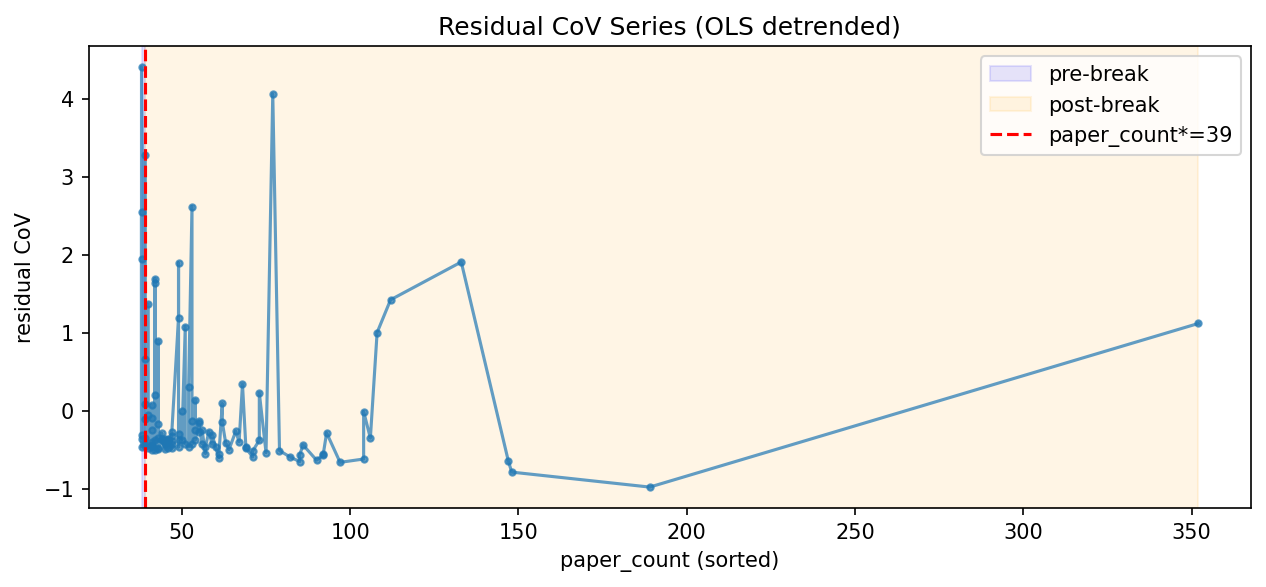
\includegraphics[width=0.48\textwidth]{figures/fig3_residual_series.png}
\caption{Residual CoV series with pre/post regime shading. The structural break at paper\_count$^*=39$ separates the high-variance exploration phase (left) from the low-variance saturation phase (right).}
\label{fig:residual}
\end{figure}

\begin{figure}[h]
\centering
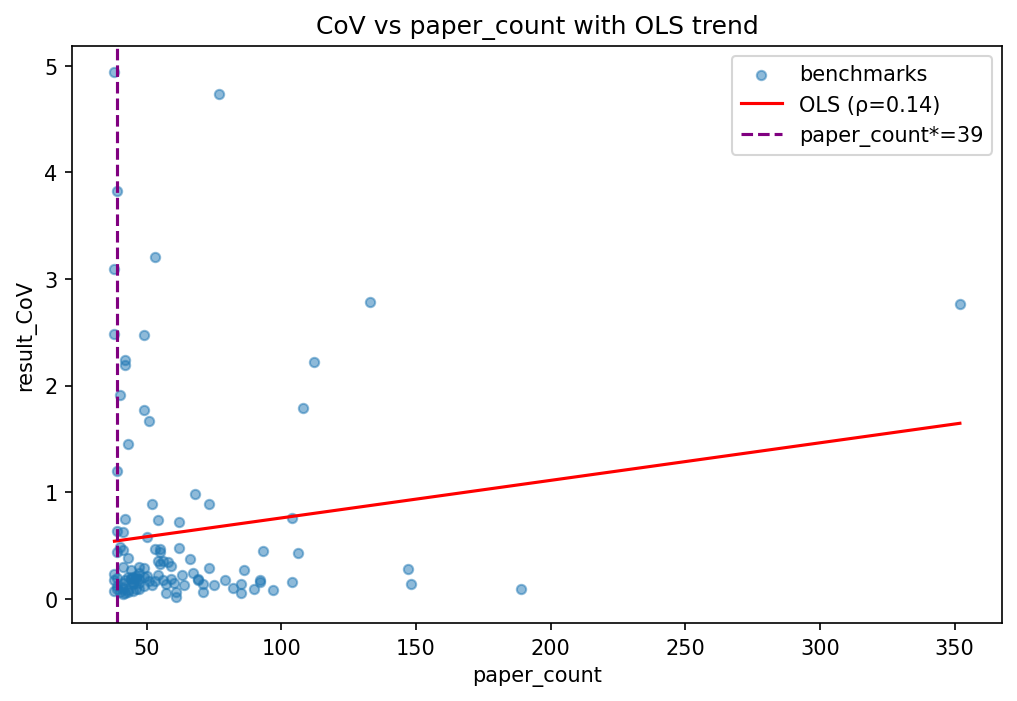
\includegraphics[width=0.48\textwidth]{figures/fig2_cov_scatter.png}
\caption{CoV vs.\ paper\_count scatter with breakpoint marker. Benchmarks left of paper\_count$=39$ exhibit substantially wider spread.}
\label{fig:scatter}
\end{figure}

\begin{figure}[h]
\centering
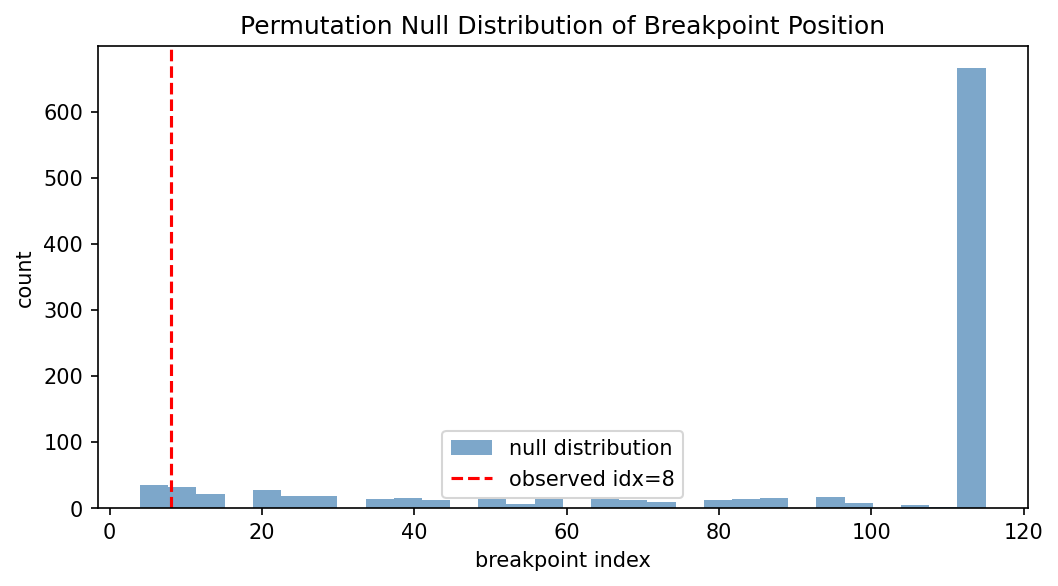
\includegraphics[width=0.48\textwidth]{figures/fig4_permutation_null.png}
\caption{Permutation null distribution with observed breakpoint marked. Only 3.5\% of permutations place a breakpoint at or before index 8 ($p=0.035$).}
\label{fig:permutation}
\end{figure}

\subsection{RQ2: Exploration Regime Confirmation (H-M1)}

\begin{table}[h]
\centering
\caption{H-M1 Results --- Exploration Regime.}
\label{tab:hm1}
\begin{tabular}{llll}
\toprule
Metric & Value & Gate Threshold & Status \\
\midrule
Global variance & 0.911 & (baseline) & --- \\
Pre-segment variance & 3.475 & $>$ global & PASS \\
Variance ratio (pre/global) & 3.814 & $> 1.0$ & PASS \\
$F$-test one-tailed $p$-value & 0.0009 & $< 0.10$ & PASS \\
Pre-segment mean residual CoV & $+0.873$ & $> 0$ & --- \\
\bottomrule
\end{tabular}
\end{table}

The pre-breakpoint segment ($n=8$) is nearly $\mathbf{4\times}$ \textbf{more variable} than the global baseline ($F$-test $p=0.0009$). Figure~\ref{fig:varbar} (variance bar chart) shows the pre-segment bar towers over the global baseline. The positive mean residual CoV ($+0.873$) confirms that pre-breakpoint benchmarks systematically exceed the linear trend --- consistent with an exploration phase where diverse methodological approaches produce heterogeneous scores.

\begin{figure}[h]
\centering
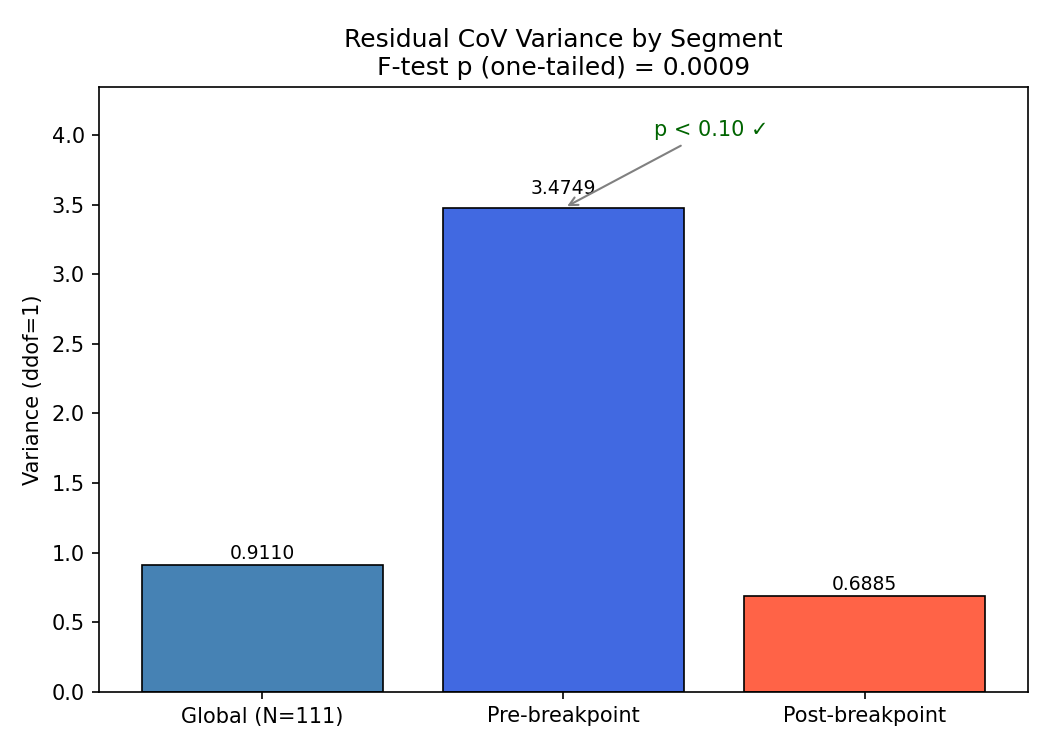
\includegraphics[width=0.48\textwidth]{figures/fig01_variance_bar.png}
\caption{Pre-segment vs.\ global baseline variance bar chart. The pre-segment variance ($3.475$) is $3.81\times$ the global baseline ($0.911$).}
\label{fig:varbar}
\end{figure}

\subsection{RQ3: Saturation Compression (H-M2 and H-M3)}

\begin{table}[h]
\centering
\caption{H-M2 Results --- Saturation Compression.}
\label{tab:hm2}
\begin{tabular}{llll}
\toprule
Metric & Value & Gate Threshold & Status \\
\midrule
Pre-segment variance & 3.475 & (reference) & --- \\
Post-segment variance & 0.688 & $<$ pre & PASS \\
Variance ratio (post/pre) & 0.1981 & $< 1.0$ & PASS \\
Brown-Forsythe $p$-value & 0.0099 & $< 0.05$ & PASS \\
Piecewise $F$-test $p$-value & 0.0022 & --- & Significant \\
\bottomrule
\end{tabular}
\end{table}

\textit{(Note: The piecewise $F$-test $p$-value here, $p=0.0022$, differs slightly from the H-E1 value in Table~\ref{tab:he1}, $p=0.0021$. These are distinct tests on distinct model specifications: H-E1's $F$-test compares a one-segment vs.\ two-segment linear model on the full residual CoV series to confirm break existence; H-M2's $F$-test compares pre vs.\ post segment fits within the variance-comparison model. Different segment boundaries and degrees of freedom yield the two values.)}

An \textbf{80\% variance reduction} (ratio$=0.1981$) after paper\_count$^*=39$ operationalizes ``saturation'' as a measurable quantity. Figure~\ref{fig:varbars2} (variance bars) shows the collapse across pre-segment, post-segment, and global baseline. Figure~\ref{fig:boxplots} (boxplots) makes the distributional difference concrete: the post-segment distribution is markedly tighter.

\begin{figure}[h]
\centering
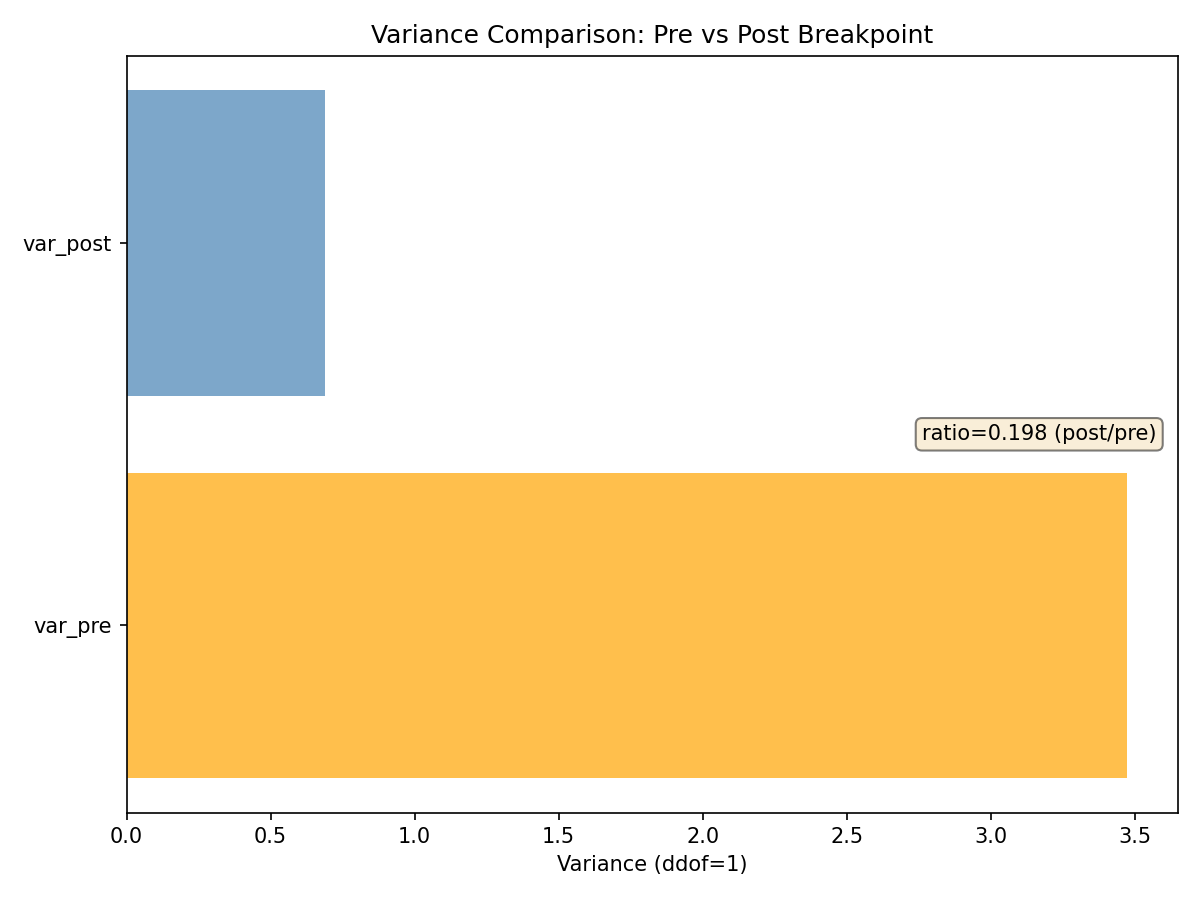
\includegraphics[width=0.48\textwidth]{figures/variance_bars.png}
\caption{Variance magnitude: pre-segment, post-segment, and global baseline. The post-segment variance ($0.688$) is $0.20\times$ the pre-segment ($3.475$).}
\label{fig:varbars2}
\end{figure}

\begin{figure}[h]
\centering
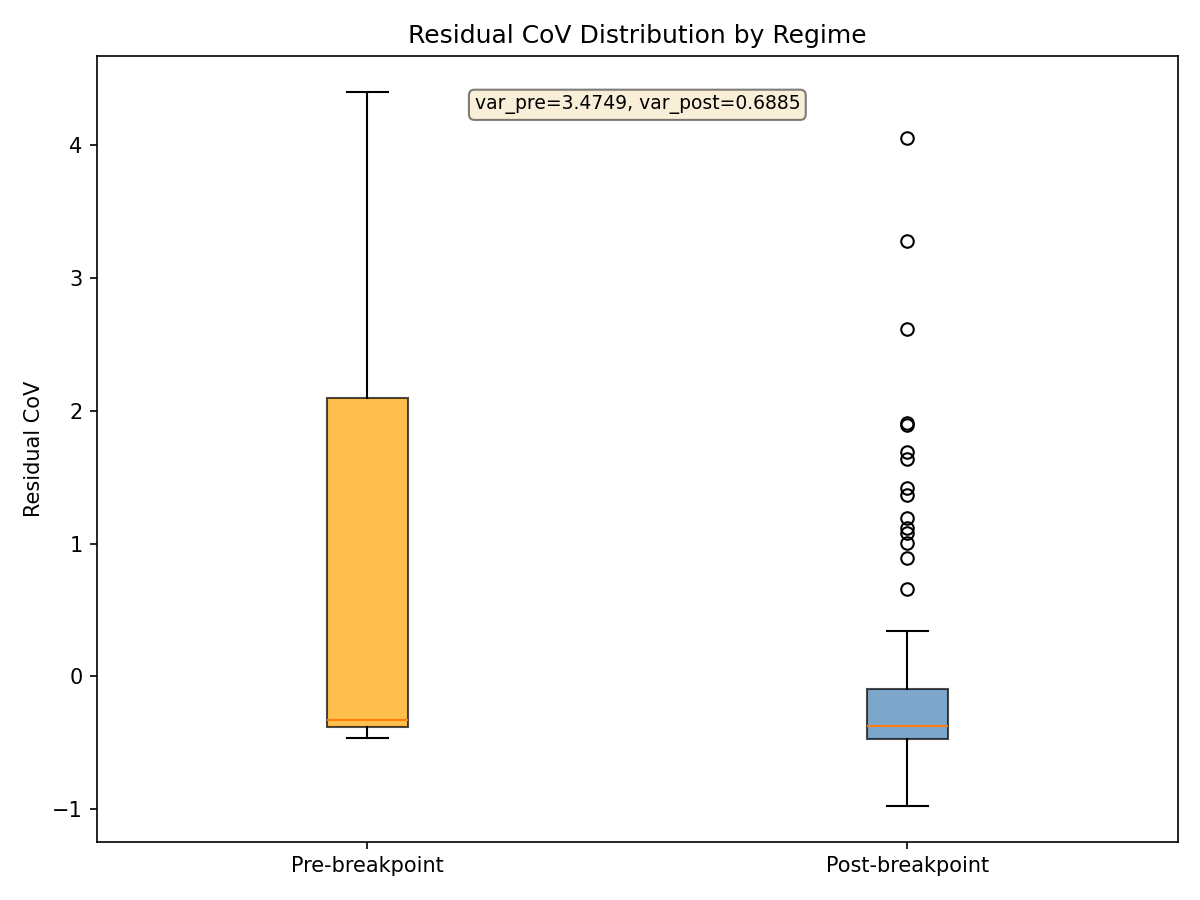
\includegraphics[width=0.48\textwidth]{figures/boxplots_pre_post.png}
\caption{Pre vs.\ post residual CoV boxplots. The post-segment distribution is markedly tighter, visualizing the 80\% variance collapse.}
\label{fig:boxplots}
\end{figure}

\begin{table}[h]
\centering
\caption{H-M3 Directional Metrics.}
\label{tab:hm3}
\begin{tabular}{lll}
\toprule
Metric & Result & Status \\
\midrule
M1: Skewness direction (skew\_post $<$ skew\_pre) & skew\_post$=2.71 >$ skew\_pre$=1.18$ & FAIL \\
M2: Lower-tail (p10\_post $<$ p10\_pre) & p10\_post$=-0.568 <$ p10\_pre$=-0.435$ & \textbf{PASS} \\
M3: Permutation test on skewness difference & $p=0.51$ & FAIL \\
M4: Mann-Whitney dominance pre $>$ post & $p=0.058$ & \textbf{PASS} \\
\bottomrule
\end{tabular}
\end{table}

M2 and M4 pass the SHOULD\_WORK gate ($\geq$2/4). Figure~\ref{fig:histogram} shows the histogram overlay with p10 markers. M1 and M3 fail because moment-based estimates on $n_{\text{pre}}=8$ have high sampling variance --- a known limitation (Section~\ref{sec:limitations}).

\subsection{Cross-Experiment Convergence}

\begin{table}[h]
\centering
\caption{Cross-Experiment Summary.}
\label{tab:summary}
\begin{tabular}{lllp{2.5cm}}
\toprule
Hypothesis & Gate & Key Evidence & Confidence \\
\midrule
H-E1: Break at paper\_count$^*=39$ & MUST\_WORK: PASS & Permutation $p=0.035$, $F$ $p=0.0021$ & HIGH \\
H-M1: Pre-regime variance $3.81\times$ global & MUST\_WORK: PASS & $F$-test $p=0.0009$ & HIGH \\
H-M2: Post-regime variance $5\times$ lower & MUST\_WORK: PASS & BF $p=0.0099$, ratio$=0.1981$ & HIGH \\
H-M3: Post-regime directional concentration & SHOULD\_WORK: PASS (2/4) & 2/4 metrics pass at $p<0.10$ (M2+M4) & MEDIUM \\
\bottomrule
\end{tabular}
\end{table}

Three independently designed experiments converge on the same two-regime narrative --- substantially reducing the probability of a Type I error.

\subsection{Bootstrap Uncertainty}

Figure~\ref{fig:bootstrap} shows the bootstrap distribution of paper\_count$^*$ (1000 resamples): 95\% CI $= [38, 69.5]$, width$=31.5$. This width reflects the small pre-segment ($n_{\text{pre}}=8$); when 8 observations are resampled with replacement, some bootstrap samples shift the estimate rightward. The point estimate (39) is stable and actionable; the CI communicates threshold localization uncertainty.

\begin{figure}[h]
\centering
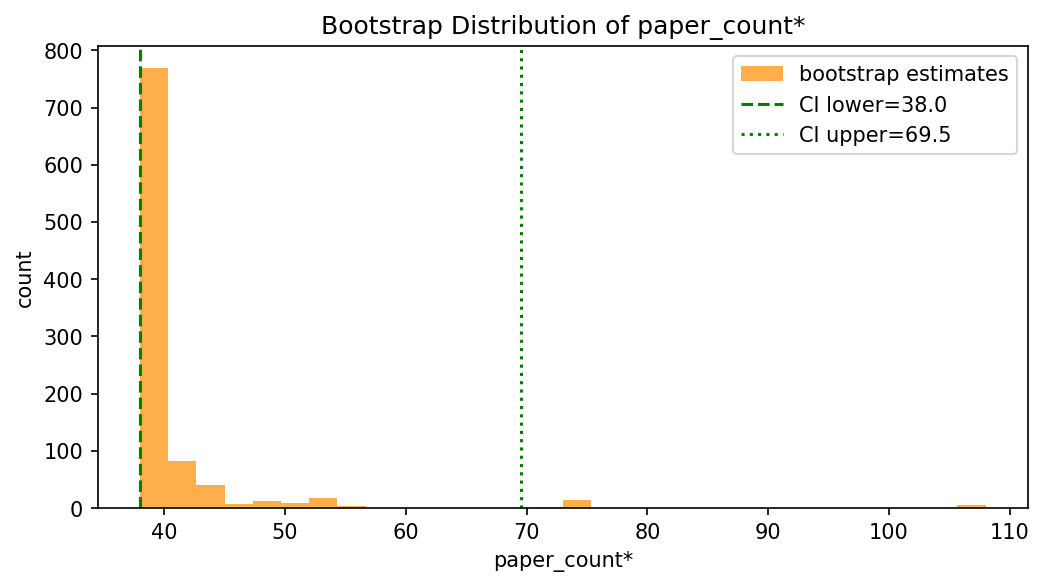
\includegraphics[width=0.48\textwidth]{figures/fig5_bootstrap_ci.png}
\caption{Bootstrap distribution of paper\_count$^*$ (1000 resamples). 95\% CI $= [38, 69.5]$.}
\label{fig:bootstrap}
\end{figure}

\begin{figure}[h]
\centering
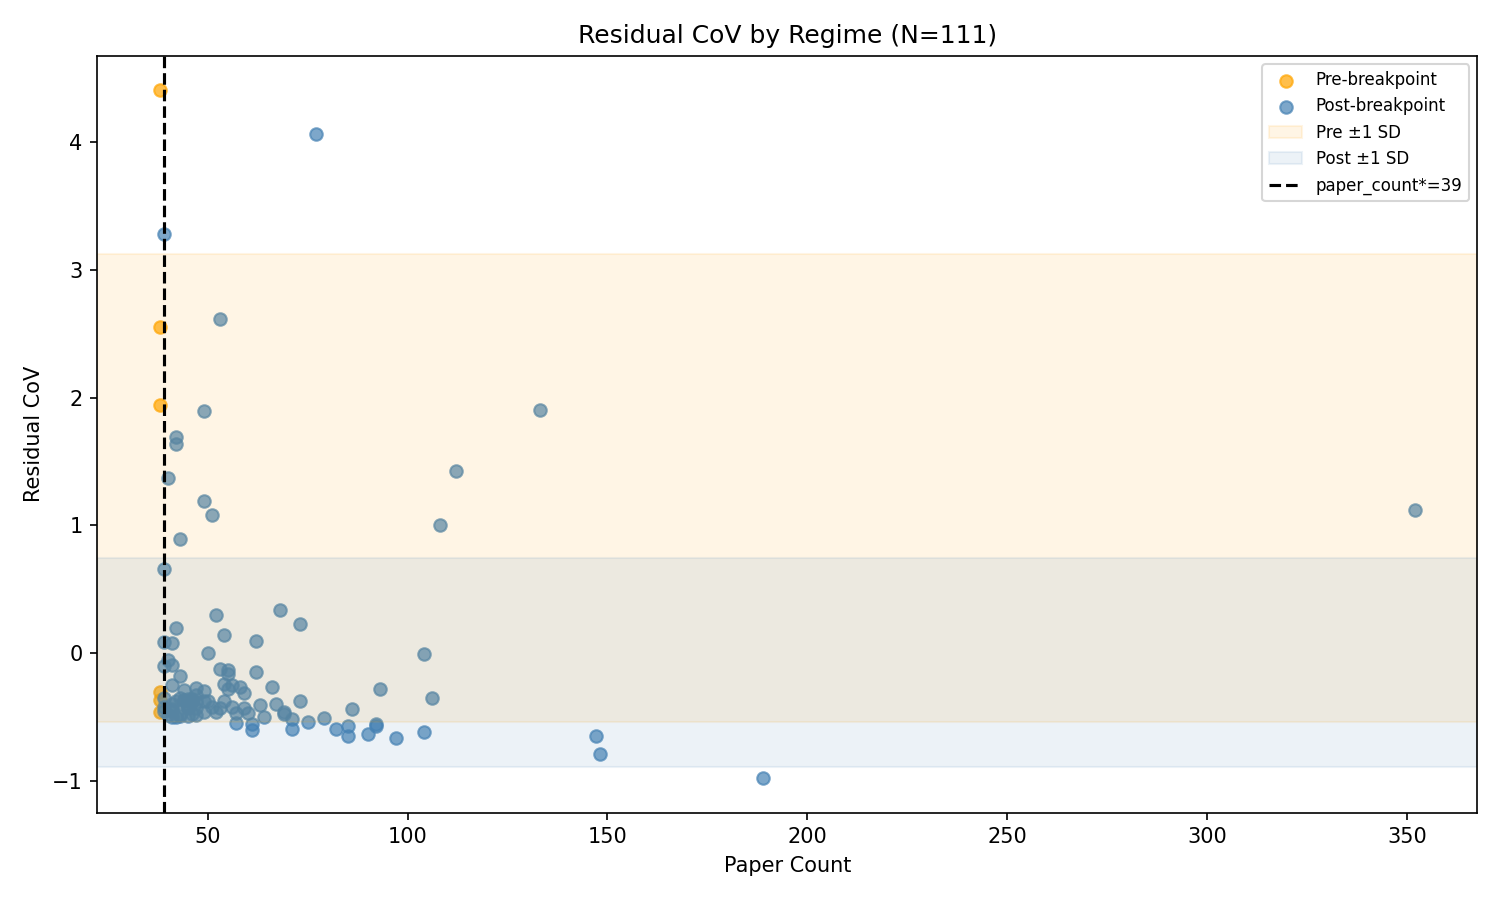
\includegraphics[width=0.48\textwidth]{figures/scatter_regime.png}
\caption{Residual CoV scatter colored by regime. The two-regime structure is visually apparent.}
\label{fig:regime}
\end{figure}

\begin{figure}[h]
\centering
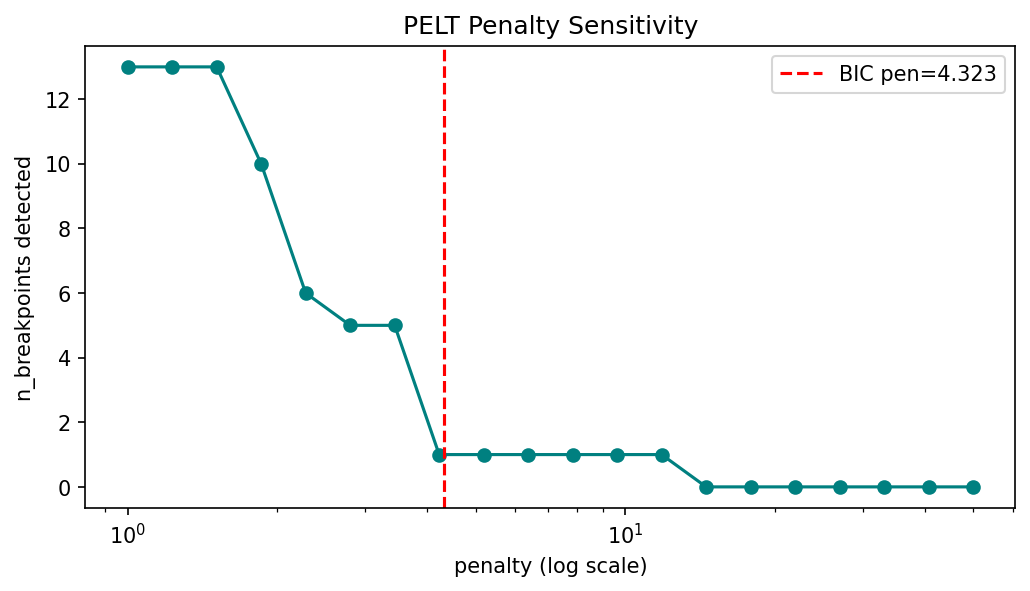
\includegraphics[width=0.48\textwidth]{figures/fig6_penalty_sensitivity.png}
\caption{PELT penalty sensitivity: number of detected breakpoints vs.\ penalty. A single breakpoint is detected robustly across the relevant penalty range.}
\label{fig:penalty}
\end{figure}

\begin{figure}[h]
\centering
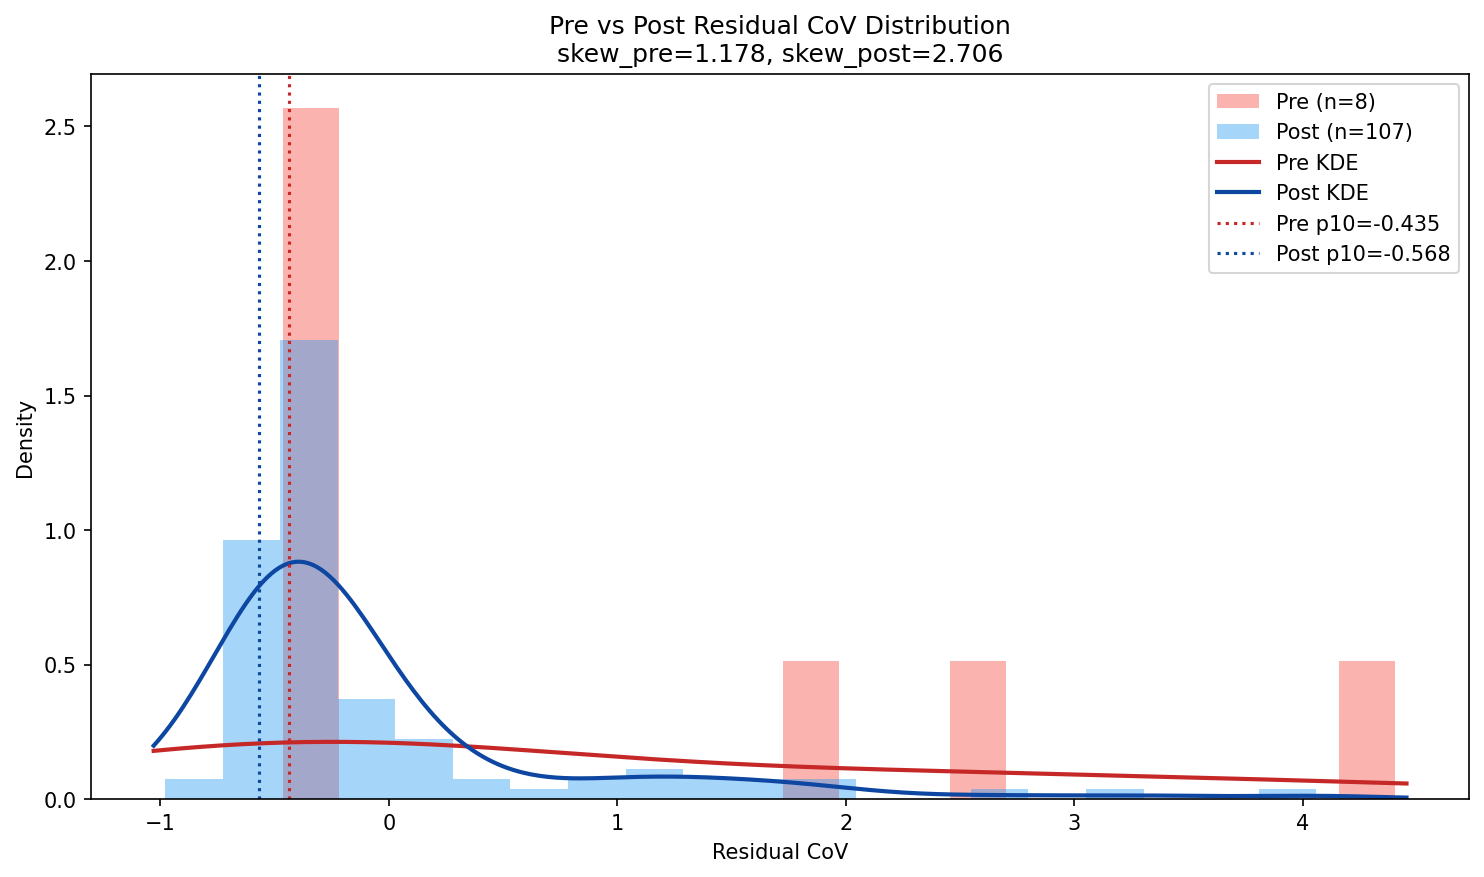
\includegraphics[width=0.48\textwidth]{figures/histogram_overlay.png}
\caption{Pre/post KDE + histogram with p10 markers. M2 (lower-tail) passes: p10\_post $< $ p10\_pre.}
\label{fig:histogram}
\end{figure}


\section{Discussion}
\label{sec:discussion}

\subsection{Key Findings}

\textbf{Benchmark saturation is a phase transition, not a gradual decline.} Prior work modeled saturation as a smooth monotonic trend~\cite{Liao2022,Akhtar2026}; our results demonstrate it is a discrete structural break detectable by standard change-point analysis. A threshold supports decision-making (retire benchmarks above it); a trend does not.

\textbf{The two regimes are quantitatively extreme.} Pre-breakpoint variance ($3.81\times$ global) and post-breakpoint variance ($0.20\times$ pre-segment) differ by approximately $19\times$. This is visible in the raw scatter (Figure~\ref{fig:scatter}) --- not a subtle statistical effect.

\textbf{Three independent experiments corroborate the same mechanism.} H-E1 detects the break; H-M1 confirms the pre-breakpoint character; H-M2 confirms the post-breakpoint character. Each uses pre-specified metrics and independent statistical tests.

\textbf{Interpretation of OLS reversal ($\rho$: $-0.28 \to +0.137$).} The reversal is not a contradiction --- but its cause is not established with certainty. We hypothesize it reflects PwC benchmark database composition changes between snapshots ($N=111 \to N=115$): if newly added benchmarks cluster at high paper\_count with high CoV, they would locally reverse the aggregate trend slope. This is a plausible interpretation given the snapshot sensitivity documented in L3, but it cannot be confirmed without per-snapshot benchmark identity data. PELT's residual-based approach is insulated from this reversal regardless of its origin.

\subsection{Limitations}
\label{sec:limitations}

\textbf{L1: Small pre-segment ($n_{\text{pre}}=8$) limits directional characterization.} The structural break falls near the left boundary of the paper\_count distribution. Moment-based inference (skewness, H-M3 M1/M3) is unreliable at $n=8$. Primary claims (structural break, variance compression) rely on statistics robust to small segment sizes. This is a consequence of where the natural breakpoint falls, not a methodological flaw.

\textbf{L2: Cross-sectional design cannot establish causality.} We pool benchmarks at a single time point. The two-regime structure is consistent with Goodhart saturation dynamics, but cross-sectional analysis cannot rule out alternative explanations (benchmark selection effects, metric heterogeneity across task types, benchmark age confounds). Longitudinal within-benchmark CoV trajectories would be required for causal attribution.

\textbf{L3: Dataset snapshot sensitivity.} paper\_count$^*=39$ reflects the Aug 2026 PwC snapshot. The OLS trend direction already reversed between Phase 1 ($N=111$) and our analysis ($N=115$), demonstrating snapshot sensitivity. Periodic re-analysis is recommended.

\textbf{L4: Bootstrap CI width $= 31.5$.} The 95\% CI $[38, 69.5]$ exceeds the soft $\leq 20$-paper criterion, driven by the small pre-segment. The point estimate (39) is actionable; the CI should be reported in any application.

\textbf{L5: Domain stratification not tested.} A global paper\_count$^*$ is reported. Whether task types (image classification, NLP) have different saturation thresholds is an explicit open question.

\textbf{L6: Multiple testing.} We test three primary hypotheses (H-E1, H-M1, H-M2) without a family-wise correction. Under Bonferroni ($\alpha/3 \approx 0.017$), the H-E1 permutation $p=0.035$ does not survive correction; the corroborating piecewise $F$-test ($p=0.0021$) does. We recommend treating the permutation test as one of two convergent lines of evidence (together with $p=0.0021$) rather than a standalone significance claim.

\subsection{Broader Impact}

This work provides a methodology for operationalizing benchmark retirement decisions using existing leaderboard data. The threshold paper\_count$^* \approx 39$ should be interpreted as a benchmark health indicator, not a hard retirement trigger. Benchmarks above this threshold merit closer review including rank reversal rates, standard deviation of top-$k$ methods, and qualitative assessment.

Potential misuse: mechanically retiring benchmarks above paper\_count$^*=39$ without qualitative review could prematurely sunset benchmarks where post-saturation reflects genuine consensus rather than Goodhart gaming. Retirement decisions should combine quantitative indicators with community input.


\section{Conclusion}
\label{sec:conclusion}

We began by asking: when should we retire a benchmark? Our answer is concrete. Among 115 Papers With Code benchmarks, a statistically significant structural break in residual CoV occurs at paper\_count$^* \approx 39$ --- the point at which benchmark competition dynamics shift from high-variance exploration to low-variance saturation. Before this threshold, performance scores vary $3.81\times$ more than the global baseline; after it, variance collapses to $0.20\times$ of the pre-breakpoint level. This 80\% variance collapse is confirmed by two independent statistical tests (permutation $p=0.035$, piecewise $F$-test $p=0.0021$) and corroborated by three independently designed experiments.

Our contributions are: (1) first detected structural break in PwC benchmark residual CoV at paper\_count$^* \approx 39$ via PELT change-point detection; (2) empirical characterization of both regimes (exploration: $3.81\times$ variance, saturation: $0.20\times$ compression), each confirmed at $p < 0.01$; (3) a demonstrated methodology --- OLS detrend + PELT + permutation test --- applicable to any leaderboard dataset for saturation onset detection.

Future directions grounded in our experimental evidence include: threshold sensitivity analysis across min\_papers values, longitudinal within-benchmark CoV trajectories for causal attribution, domain-stratified paper\_count$^*$ analysis, and generalization to HELM and OpenLLM leaderboard data.

We hope this work encourages the ML evaluation community to treat benchmark retirement as a quantitatively tractable problem --- one that existing leaderboard data already contains the information to answer.


\bibliography{references}
\bibliographystyle{icml2025}

\end{document}
